\documentclass[a4paper,11pt]{article}
\usepackage[utf8]{inputenc}
\usepackage[usenames,dvipsnames]{color}
\usepackage{graphicx}
\usepackage[justification=centering,labelfont=bf]{caption}
\usepackage{listings}
\usepackage{minted}
\usepackage[hidelinks]{hyperref}
\begin{document}
\begin{titlepage}
\begin{center}
\textsc{\Large Parallelism}
\\
\texttt{1202}
\\[1.5cm]
\rule{\linewidth}{0.5mm}
\\[0.4cm]
{\huge
\bfseries
Lab 2: Geometric decomposition – solving the heat equation
\\[0.4cm]
}
\rule{\linewidth}{0.5mm}
\\[2.5cm]
\begin{minipage}{0.4\textwidth}
\begin{flushleft}
\large
Héctor Ramón Jiménez
\end{flushleft}
\end{minipage}
\begin{minipage}{0.4\textwidth}
\begin{flushright}
\large
Alvaro Espuña Buxo
\end{flushright}
\end{minipage}
\vfill
{\large
\today
}
\\
{\large
\texttt{Facultat d'Informàtica de Barcelona}
}
\end{center}
\end{titlepage}
\section{Analysis of dependences for the heat equation}
The analysis of the dependencies caused by the proposed task
decomposition for the two solvers of the heat equation has been done
using Tareador. Dependences appear when a task reads a memory position
previously written by another task. Some dependences may impose task
ordering constraints while other may impose data access
constraints. For solving the heat equation two different solvers have
been used, each with different dependence patterns.

For the Jacobi solver, there are two data dependencies between
iterations, \texttt{sum} and \texttt{diff}. \texttt{diff} is not a
real dependency, because it's value is not reused, but it's a global
variable. \texttt{sum} presents the tipical acumulator dependence
pattern. This dependences are only data-access dependences. Note that,
to update the value in a cell we need to read its neighbours, but then
we write the new value in a different matrix, so there's no task
ordering dependence. This can be seen in figure \ref{fig:j-deps}. In
the parallelization with OpenMP, we plan to guarantee these
dependences using an \texttt{omp pragma} with \texttt{private} for
\texttt{diff} and a reduction on \texttt{sum}.
\begin{figure}[h!]
  \includegraphics[width=1.0\textwidth]{figs/dependencies_j.pdf}
  \caption{After isolating sum in \texttt{Tareador}, a Jacobi
    iteration is fully parallelizable.}
  \label{fig:j-deps}
\end{figure}

For the Gauss-Seidel solver the dependences are a bit more complicated
(as we can see in figure \ref{fig:gs-deps}). First of all, we have a
task ordering dependence. We are reusing the same matrix, and since we
are reading all neighbours to update the current cell, we need to be
careful about the order the calculations are performed. Also, there
are data access dependences, because \texttt{unew}, \texttt{sum} and
\texttt{diff} variables are global to the parallel zone. To solve the
first part, we will use blocking. A block will be processed only when
the upper block and the block of the left have been processed. This
allows us to create individual parallelizable tasks. For the second
part, we will use \texttt{reduce} on \texttt{sum} and \texttt{private}
on \texttt{diff} and \texttt{unew}.

\begin{figure}[h!]
  \center
  \includegraphics[height=10cm,clip=true,trim=0cm 2cm 9cm 0cm]{figs/dependencies_gs.pdf}
  \caption{After isolating sum in tareador, a Gauss-Seidel iteration
    depends on the \emph{left} and \emph{upper} tasks.}
  \label{fig:gs-deps}
\end{figure}

\newpage
The following table summarizes the predicted speed–up for the parallel
execution for the two solvers, with 2, 4, 8 and 16 processors with
respect to the simulation with just 1 processor:

\begin{figure}[h!]
\begin{tabular}{| c || c | c | c | c | c |}
\hline
\textbf{\textbf{Solver}} & \textbf{2 threads} & \textbf{4 threads} & \textbf{8 threads} & \textbf{16 threads}
\\
\hline
\hline
\textbf{Jacobi} & 1.955 & 3.419 & 5.467 & 6.868
\\
\hline
\textbf{Gauss-Seidel} & 1.774 & 2.498 & 2.498 & 2.498
\\
\hline
\end{tabular}
\caption{Speed up expected. Simulated using \texttt{Paraver}.}
\label{speed-up}
\end{figure}

We can see in figure \ref{speed-up} how we expect Jacobi to scale
reasonably well, but for Gauss-Seidel, because of the data
dependencies, using with the same granularity, we won't be able to get
more speed-up adding more processors (we are bounded by the critical
path).
\newpage
\section{OpenMP parallelization and execution analysis}
\begin{enumerate}
\setcounter{enumi}{0}
\item
\textbf{Briefly comment the parallelization with OpenMP that has been
  done for the two solvers.}

First of all, for the Jacobi solver, we optimized the sequential code
to obtain almost 1.5x speed-up. Instead of performing a copy of the
matrix every time, we just swap the pointers of the struct, so it's now done
in constant time. Then, to allow parallelization we added \texttt{\#pragma
  omp} \texttt{parallel} \texttt{for} \texttt{private(diff)}
\texttt{reduction(+:sum)} before the first loop, thus solving the
dependencies between loops. Following the specification of the
assignment, we changed \texttt{nbx} to be the number of threads and
\texttt{nby} to 1, hence executing the whole matrix row with the same
thread. Because the default distribution is \texttt{static} 1, and
there will be \texttt{nbx} threads, every thread will take a \emph{row
  block}.

For the Gauss-Seibel we did more work, because there are more
dependencies.  The first thing we did was adding \texttt{\#pragma omp
  parallel for private(diff, unew) reduction(+:sum)} before the first
loop. To avoid starting on a block whose dependencies have not been
calculated we created an array (processed) that stores in the
\emph{i}-th position the greatest index of the \emph{column block}
that has been already treated by the thread \emph{i}.

\begin{minted}{c}
  int *processed = malloc(num_threads * sizeof(int));

  #pragma omp parallel for
  for (int i = 0; i < num_threads; i++)
    processed[i] =  -1;

  // ...
  int thread_id = omp_get_thread_num();
  for (int jj=0; jj<nby; jj++) {
    while (thread_id > 0 && processed[thread_id - 1] < jj) {
      #pragma omp flush(processed)
    }
    // ...
    processed[thread_id] = jj;
    #pragma omp flush(processed)
  }
  // ...
\end{minted}

We do an active wait if the previous needed block has not been processed
yet. The flush is needed to comunicate the changes in \texttt{processed}, otherwise
we would be trapped in an infinite loop.

\setcounter{enumi}{1}
\item
\textbf{Plot the speedup achieved by the OpenMP parallel version, with
  respect to sequential execution time, for the two solvers. Comment
  the results that are obtained and justify the scalability that is
  obtained. Include Paraver timelines in order to support your
  explanation.}  \setcounter{enumi}{2}

In figures \ref{fig:j-plot} and \ref{fig:gs-plot} we can see how
Jacobi scales better than Gauss-Seidel. This is because, Jacobi is
fully parallelizable and Gauss-Seidel has to be computed \emph{diagonally}.
Gauss-Seidel's speedup converges rapidly to 2.5.

Also is interesting to note that Jacobi performs better with 8 threads
than with 16.  This is because we only have 12 cores, so using 16
threads we are relying on hyperthreading.

\begin{figure}[h!]
  \center
  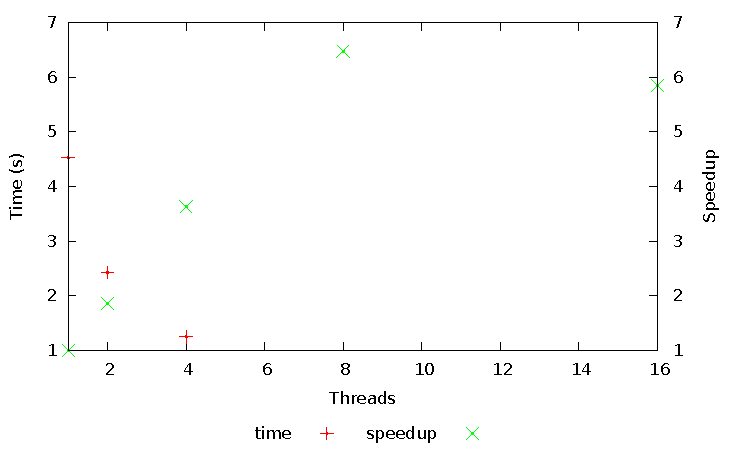
\includegraphics[width=1.0\textwidth]{figs/plot_j.pdf}
  \caption{Jacobi parallelization results.}
  \label{fig:j-plot}
\end{figure}

\begin{figure}[h!]
  \center
  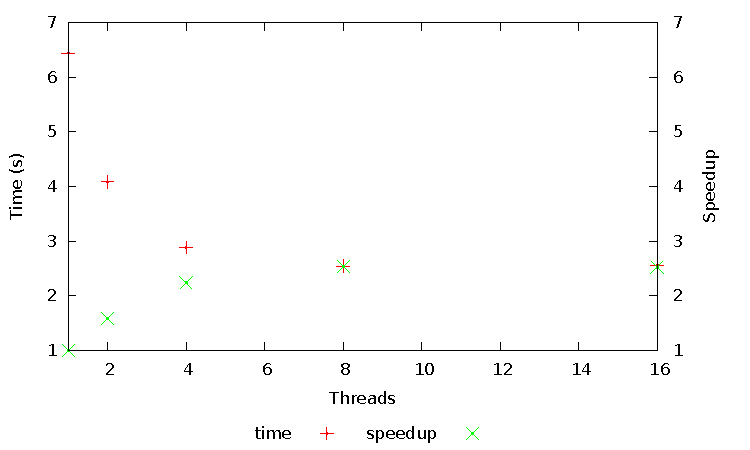
\includegraphics[width=1.0\textwidth]{figs/plot_gs.pdf}
  \caption{Gauss-Seidel parallelization results.}
  \label{fig:gs-plot}
\end{figure}

\begin{figure}[h!]
  \center
  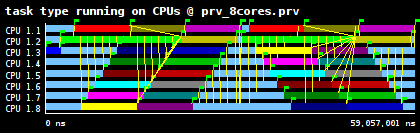
\includegraphics[width=0.7\textwidth]{figs/j_8cores.png}
  \caption{Jacobi \texttt{Paraver} simulation with 8 cores.}
  \label{fig:j-simul}
\end{figure}

\begin{figure}[h!]
  \center
  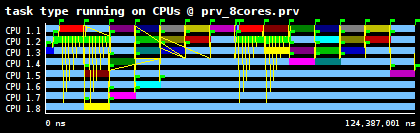
\includegraphics[width=0.7\textwidth]{figs/gs_8cores.png}
  \caption{Gauss-Seidel \texttt{Paraver} simulation with 8 cores.}
  \label{fig:gs-simul}
\end{figure}

In figures \ref{fig:j-simul} and \ref{fig:gs-simul} we can confirm using
\texttt{Paraver} that Gauss-Seidel, due to task ordering dependences,
some threads spend a lot of time idle. In Jacobi version, though, the
parallelization exploits better the multicore usage.


During this exercise we noticed that past 16 threads (17 or more), because of the
accuracy of floating point arithmetic, the results were wrong. Both
using Jacobi and Gauss-Seidel stopped earlier than expected: the
program did less iterations than the original. One possible solution
would be to adjust the threshold as a function of the number of
threads.

\clearpage
\item
\textbf{In the parallelization of Gauss-Seidel, analyze the impact on
  the parallel execution time of the block size \texttt{by} (or
  equivalently the number of blocks \texttt{nby})
    \footnote{The resulting image should be the same.}. For example
    try with \texttt{nby=2*nbx, nby=4*nbx, ...} Is there any
    performance impact? Is there an optimal point?  Justify your
    answer.}
\begin{figure}[h!]
\begin{tabular}{| l || c | c | c | c | c |}
\hline
\textbf{\texttt{nby}} & \textbf{1 thread} & \textbf{2 threads} & \textbf{4 threads} & \textbf{8 threads} & \textbf{16 threads}
\\
\hline
\hline
\texttt{2*nbx} & 6.452 & 4.051 & 2.311 & 1.421 & 1.454
\\
\hline
\texttt{4*nbx} & 6.433 & 3.597 & 1.980 & 1.275 & 1.585
\\
\hline
\texttt{8*nbx} & 6.117 & 3.211 & 1.689 & 1.375 & 2.369
\\
\hline
\texttt{16*nbx} & 5.708 & 2.763 & 1.666 & 1.678 & 3.784
\\
\hline
\texttt{32*nbx} & 4.905 & 2.642 & 1.805 & 2.629 & -
\\
\hline
\end{tabular}
\caption{Impact of the number of blocks \texttt{nby}. Time is in seconds.}
\end{figure}
\\
The number of blocks \texttt{nby} has an obvious performance
impact, affecting considerably the parallel execution times. This is
because the \texttt{nby} value is directly related with the number of
performed flushes. There are going to be at least \texttt{nby*nbx}
flushes to mark each block as processed. To this flushes we have to
add the flushes that each thread performs when it's waiting its
dependencies to be processed. Thus, the optimal value is going to be
one that finds a balance between these two types of flushes (one that
keeps \texttt{nby} reasonably low but allowing to solve the
dependencies quickly). In the obtained results this value seems to be
\texttt{4*nbx} with $8$ threads.
\end{enumerate}
\end{document}
